\documentclass{article}

\usepackage[a4paper, total={7in, 9in}]{geometry}
\pagestyle{empty} % Prevent relative page numbers

%%%%%%%%%%%%%%%%%%%%%%%%%%%%%%%%%%%%%%
%% Default definitions 
%% Define listings format
\usepackage{xcolor} % Required for listings color definitions
\definecolor{Brown}{cmyk}{0,0.81,1,0.60}
\definecolor{OliveGreen}{cmyk}{0.64,0,0.95,0.40}
\definecolor{CadetBlue}{cmyk}{0.62,0.57,0.23,0}
\definecolor{lightlightgray}{gray}{0.9}

\usepackage{listings} % computer code language formatting

\lstdefinestyle{tex-style} {
	language=[LaTeX]TeX,                    % Code langugage
	basicstyle=\ttfamily,                   % Code font, Examples: \footnotesize, \ttfamily
	%keywordstyle=\color{OliveGreen},        % Keywords font ('*' = uppercase)
	commentstyle=\color{gray},              % Comments font
	numbers=none,                           % Line nums position
	numberstyle=\tiny,                      % Line-numbers fonts
	stepnumber=1,                           % Step between two line-numbers
	numbersep=5pt,                          % How far are line-numbers from code
	backgroundcolor=\color{lightlightgray}, % Choose background color
	frame=single,                             % A frame around the code
	tabsize=2,                              % Default tab size
	captionpos=b,                           % Caption-position = bottom
	breaklines=true,                        % Automatic line breaking?
	breakatwhitespace=false,                % Automatic breaks only at whitespace?
	showspaces=false,                       % Dont make spaces visible
	showtabs=false,                         % Dont make tabls visible
	columns=flexible,                       % Column format
	morekeywords={__global__, __device__}  % CUDA specific keywords
}
\lstnewenvironment{latex}
{\lstset{language=[LaTeX]TeX}}
{}
\lstset{style=tex-style}

%% Define URL format
\usepackage[hyphens]{url}
\usepackage{hyperref}
\hypersetup{
	colorlinks=true,
	citecolor=black,
	filecolor=black,
	linkcolor=blue,
	urlcolor=blue
}

\setlength\parindent{0pt}


%%%%%%%%%%%%%%%%%%%%%%%%%%%%%%%%%%%%%%
%% Example-specific packages
\usepackage{graphicx}
\usepackage{wrapfig}
\usepackage{lipsum}  % generates filler text

%%%%%%%%%%%%%%%%%%%%%%%%%%%%%%%%%%%%%%
%% Example-specific preamble

\begin{document}

\section*{Figure Wrapping}

\subsection*{Description}
Wrapping a figure around text isn't a stock functionality in \LaTeX, but the \verb|wrapfig| package provides a clean interface for that purpose.

\subsection*{Sources}
\url{https://tex.stackexchange.com/questions/118602/how-to-text-wrap-an-image-in-latex}\\
Frog image from: \url{http://animal-wildlife.blogspot.gr/2011/08/tree-frog.html}

\subsection*{Used Packages}
\verb|wrapfig, graphicx|

\subsection*{Preamble}
\begin{latex}
%%%%%%%%%%%%%%%%%%%%%%%%%%%%%%%%%%%%%%
%% Example-specific packages
\usepackage{graphicx}
\usepackage{wrapfig}
\usepackage{lipsum}  % generates filler text

%%%%%%%%%%%%%%%%%%%%%%%%%%%%%%%%%%%%%%
%% Example-specific preamble
\end{latex}

\subsection*{Document}
\begin{latex}
{\centering
	{\Large Figure Wrapping Example}\\
	\vspace{5pt}
	{\large writeLaTeX}\\
	\vspace{5pt}
	\today\\
	\vspace{5pt}
}

\begin{wrapfigure}{R}{0.3\textwidth}
	\centering
	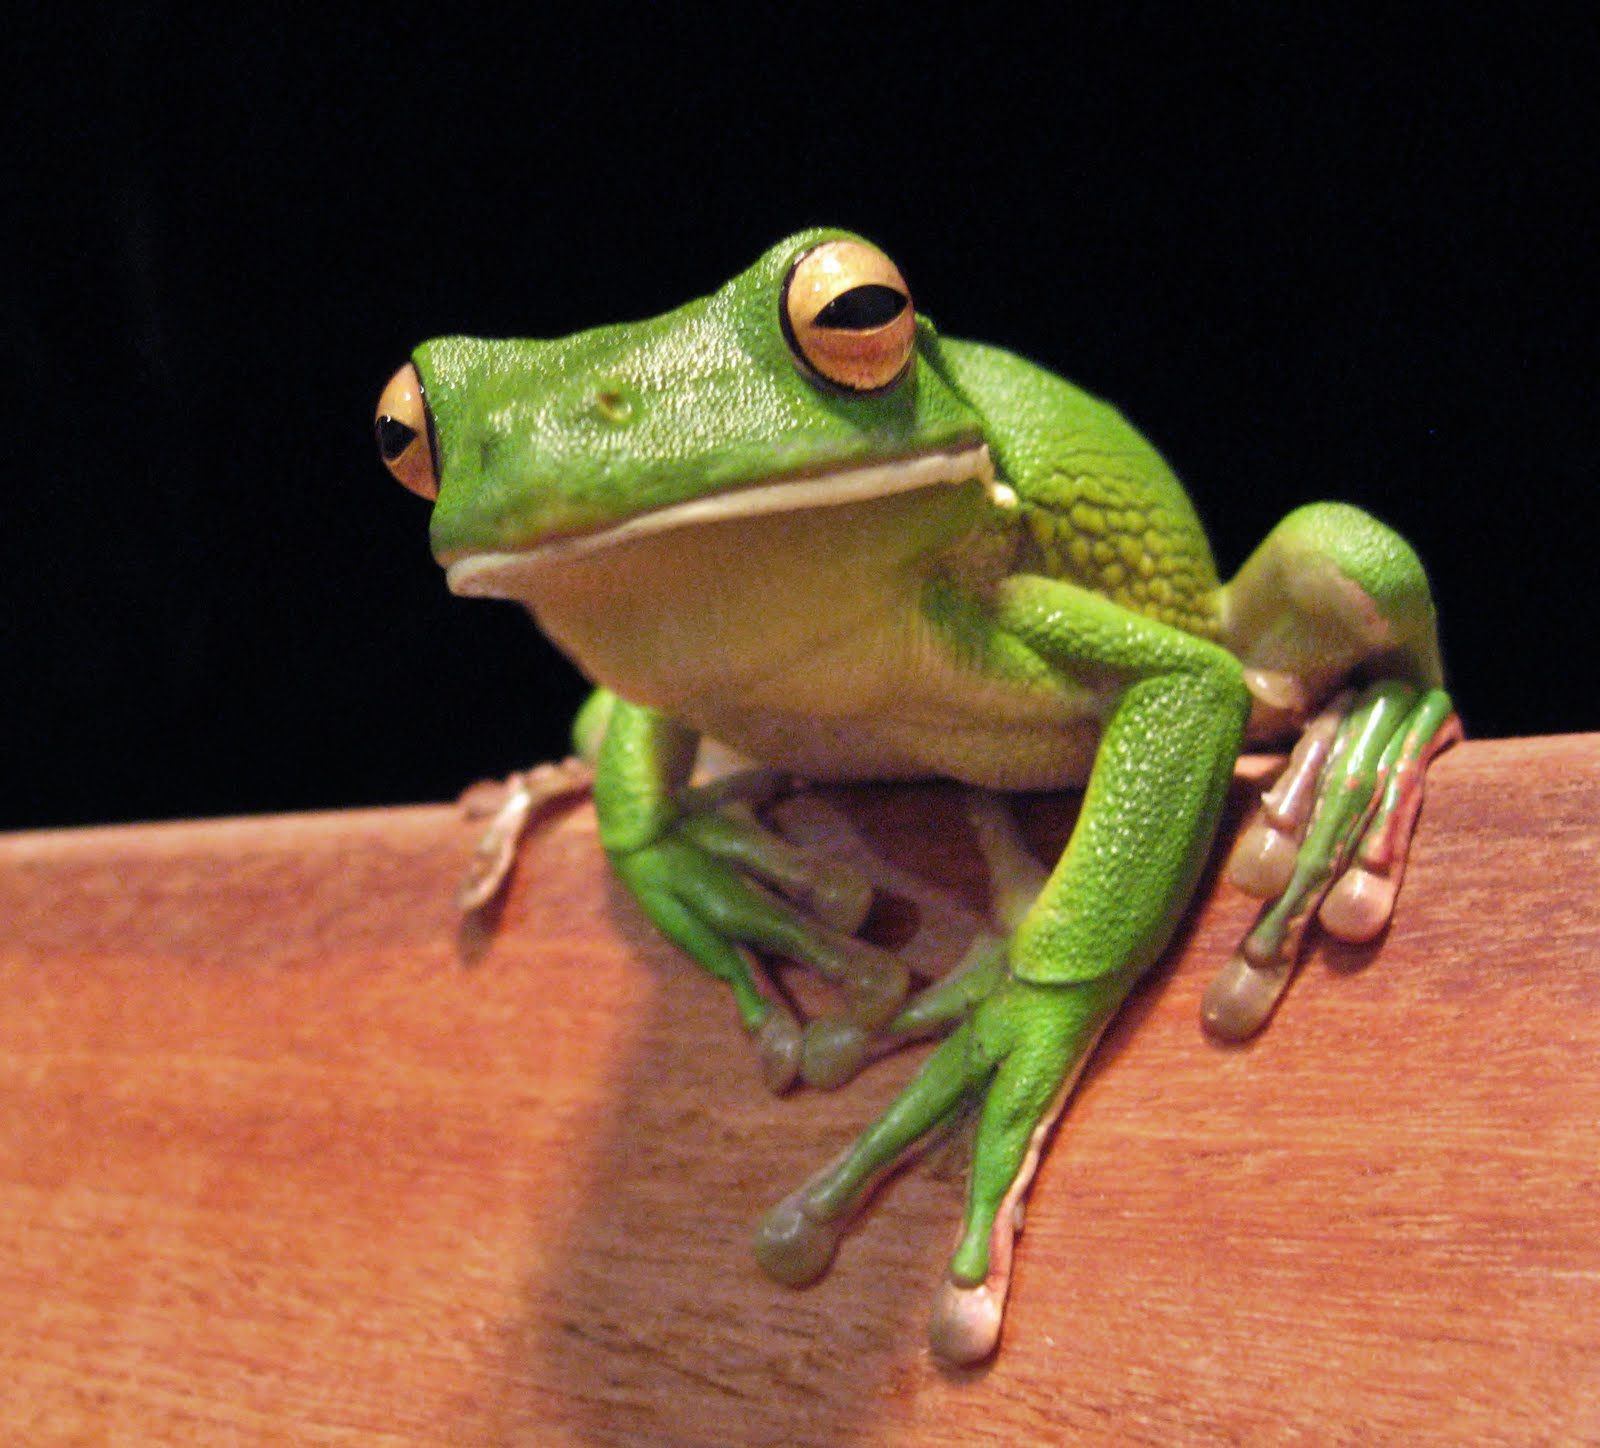
\includegraphics[width=0.25\textwidth]{frog.jpg}
	\caption{\label{fig:frog1}This is a figure caption.}
\end{wrapfigure}

\lipsum[1]

\begin{wrapfigure}{L}{0.3\textwidth}
	\centering
	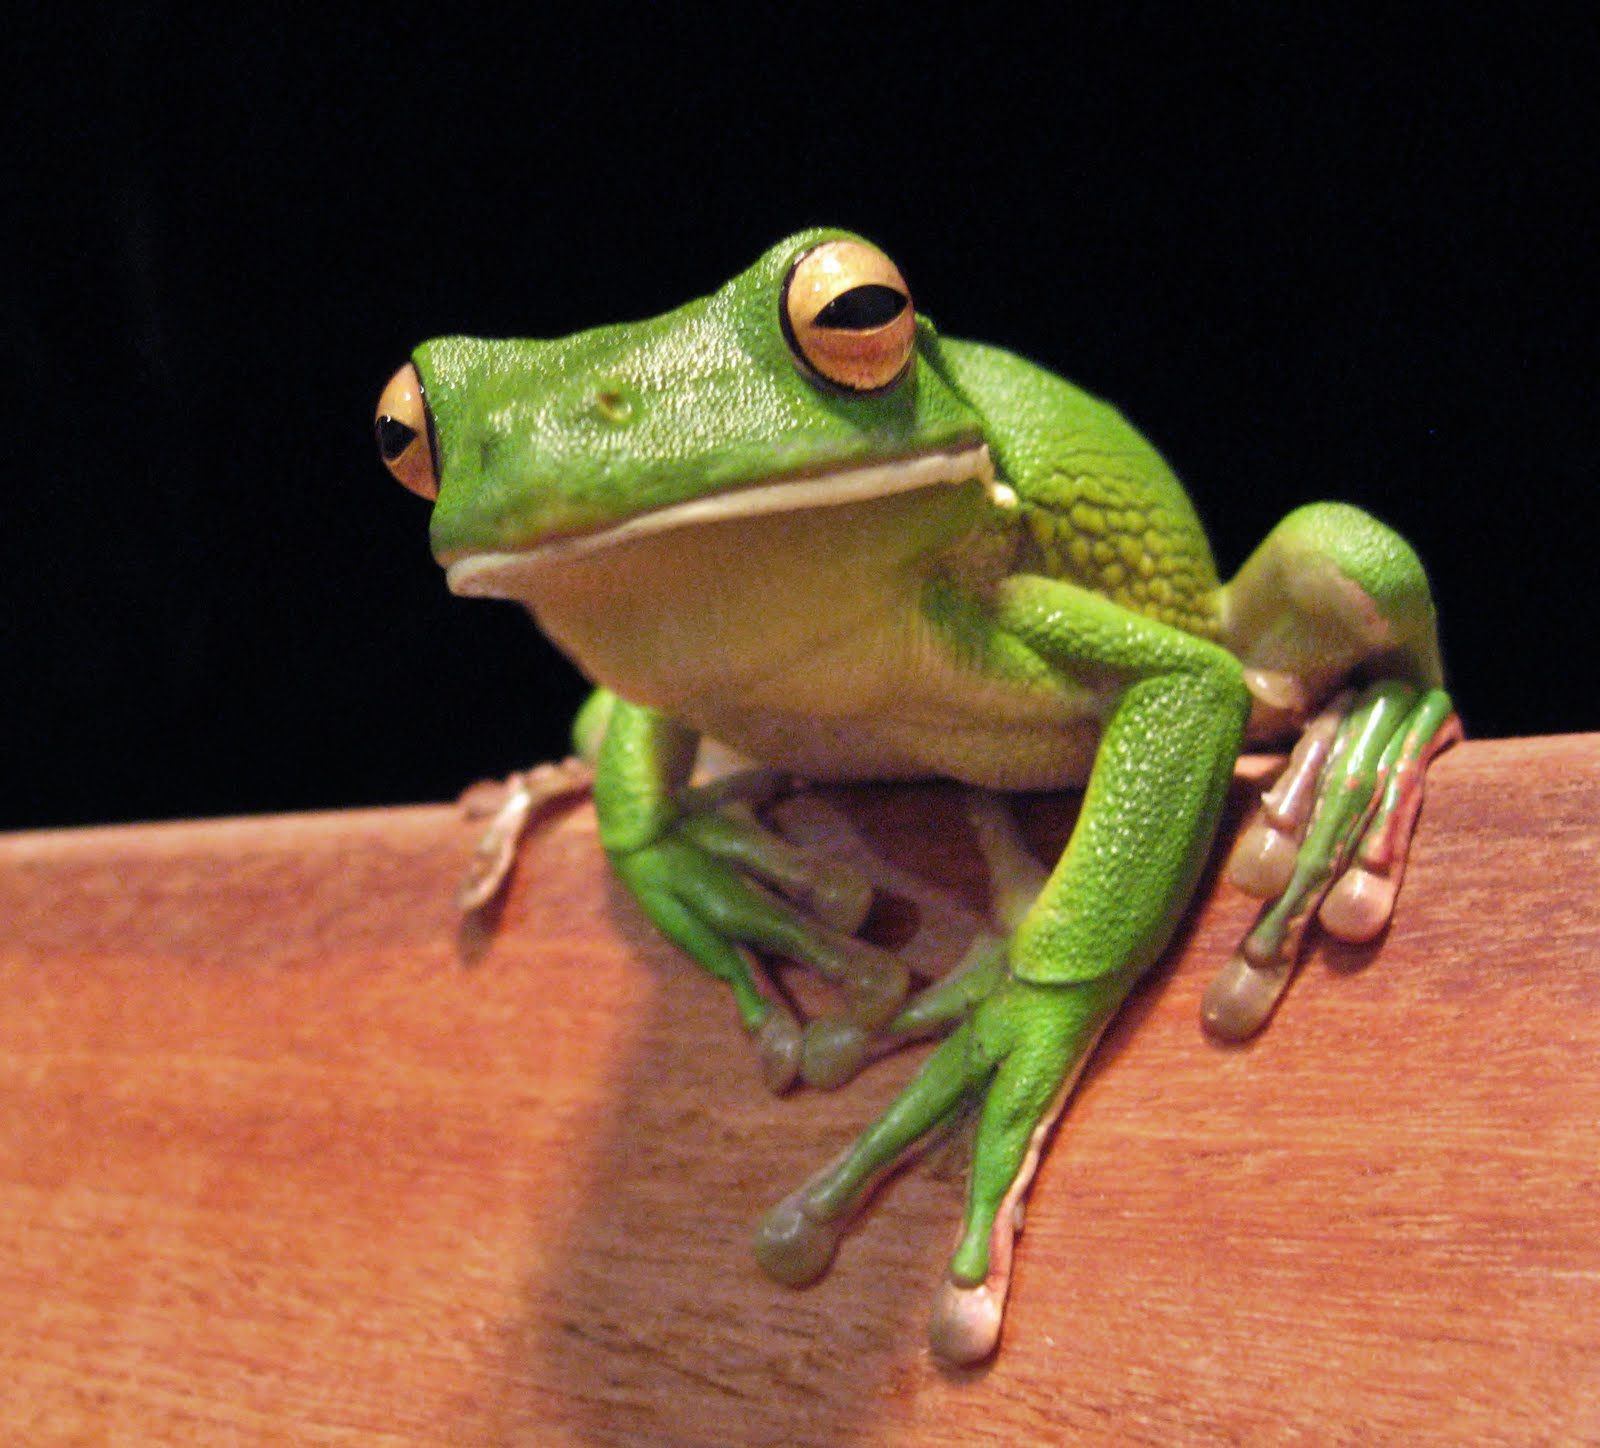
\includegraphics[width=0.25\textwidth]{frog.jpg}
	\caption{\label{fig:frog2}This is a figure caption.}
\end{wrapfigure}

\lipsum[2-3]
\end{latex}

\clearpage
\subsection*{Result}
{\centering
{\Large Figure Wrapping Example}\\
\vspace{5pt}
{\large writeLaTeX}\\
\vspace{5pt}
\today\\
\vspace{5pt}
}

\begin{wrapfigure}{R}{0.3\textwidth}
	\centering
	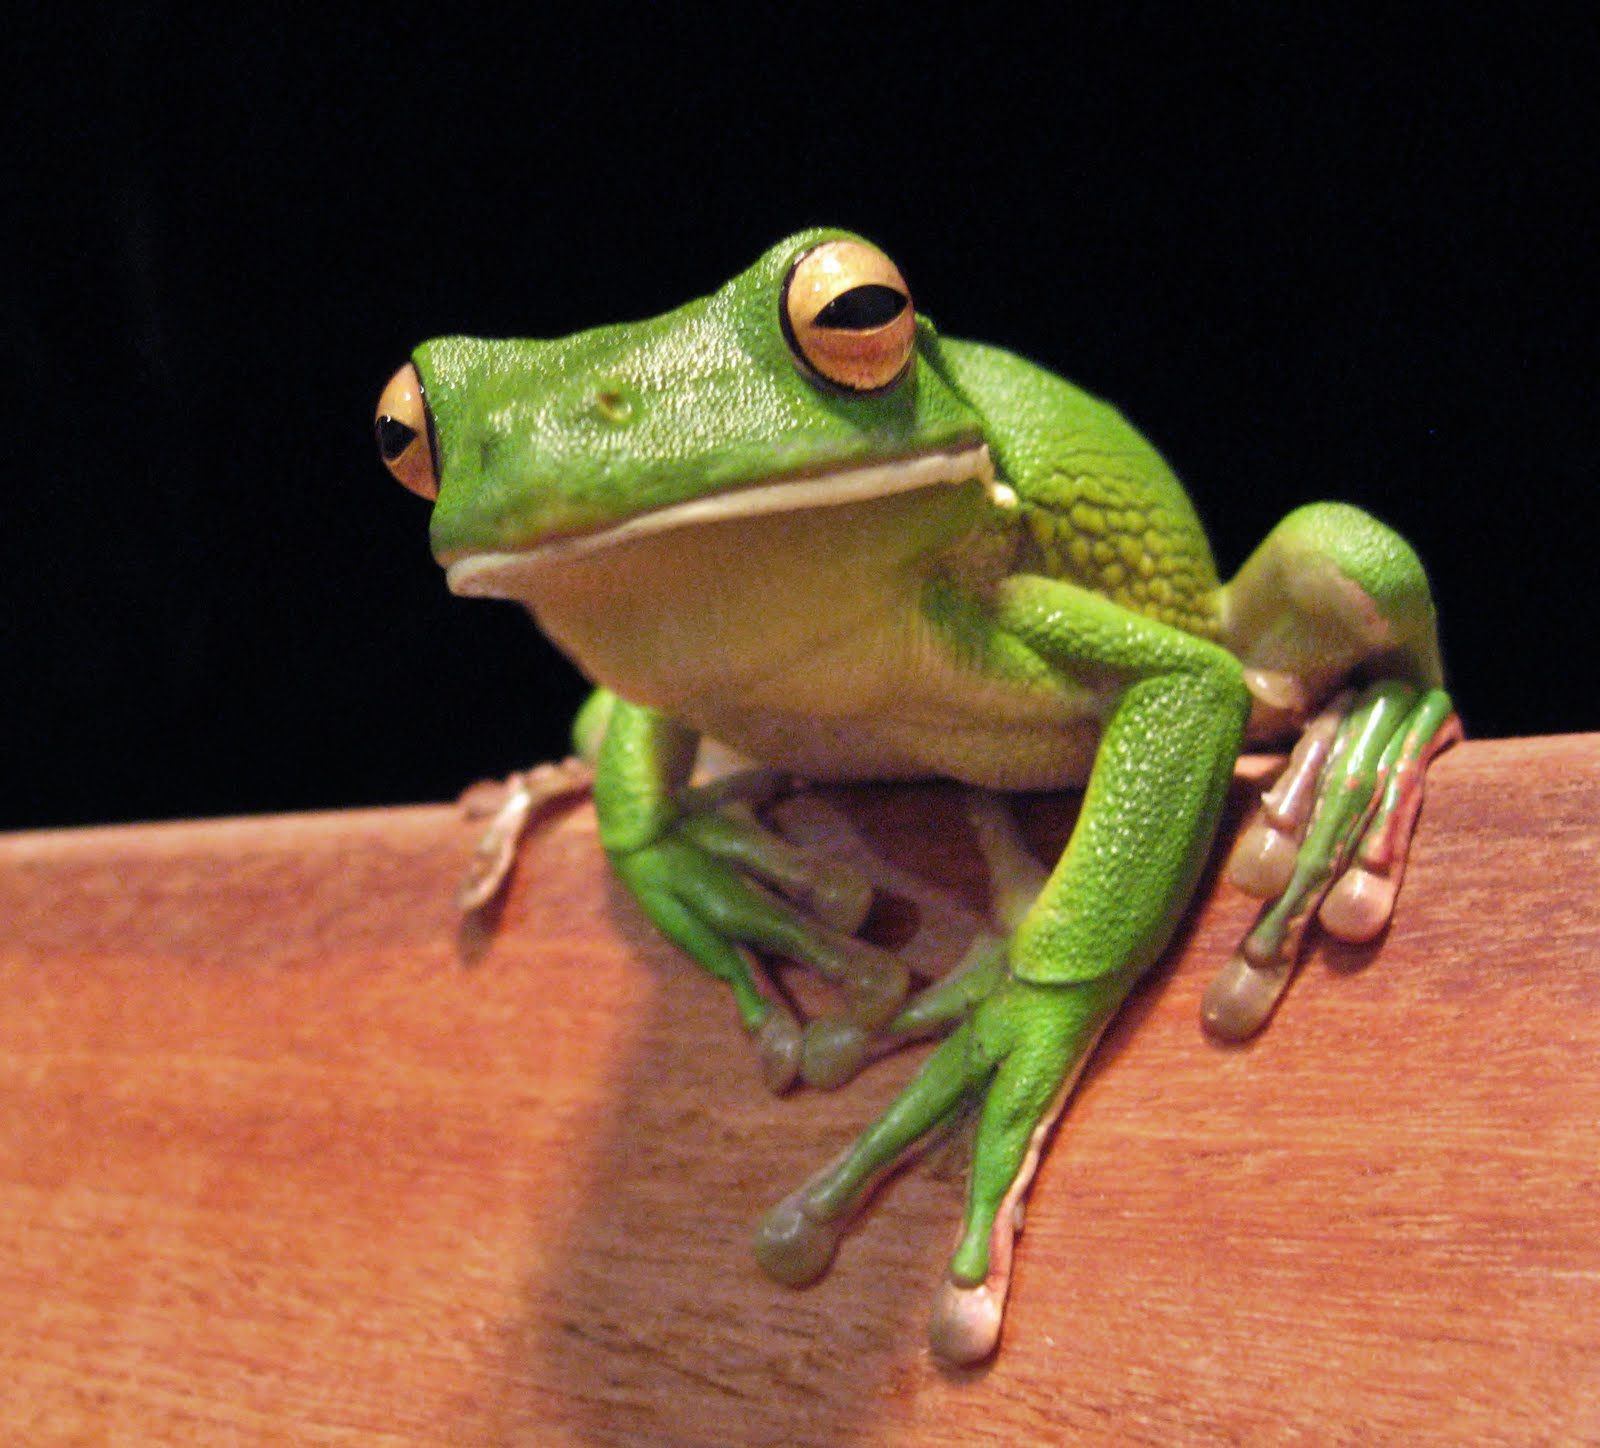
\includegraphics[width=0.25\textwidth]{frog.jpg}
	\caption{\label{fig:frog1}This is a figure caption.}
\end{wrapfigure}

\lipsum[1]

\begin{wrapfigure}{L}{0.3\textwidth}
	\centering
	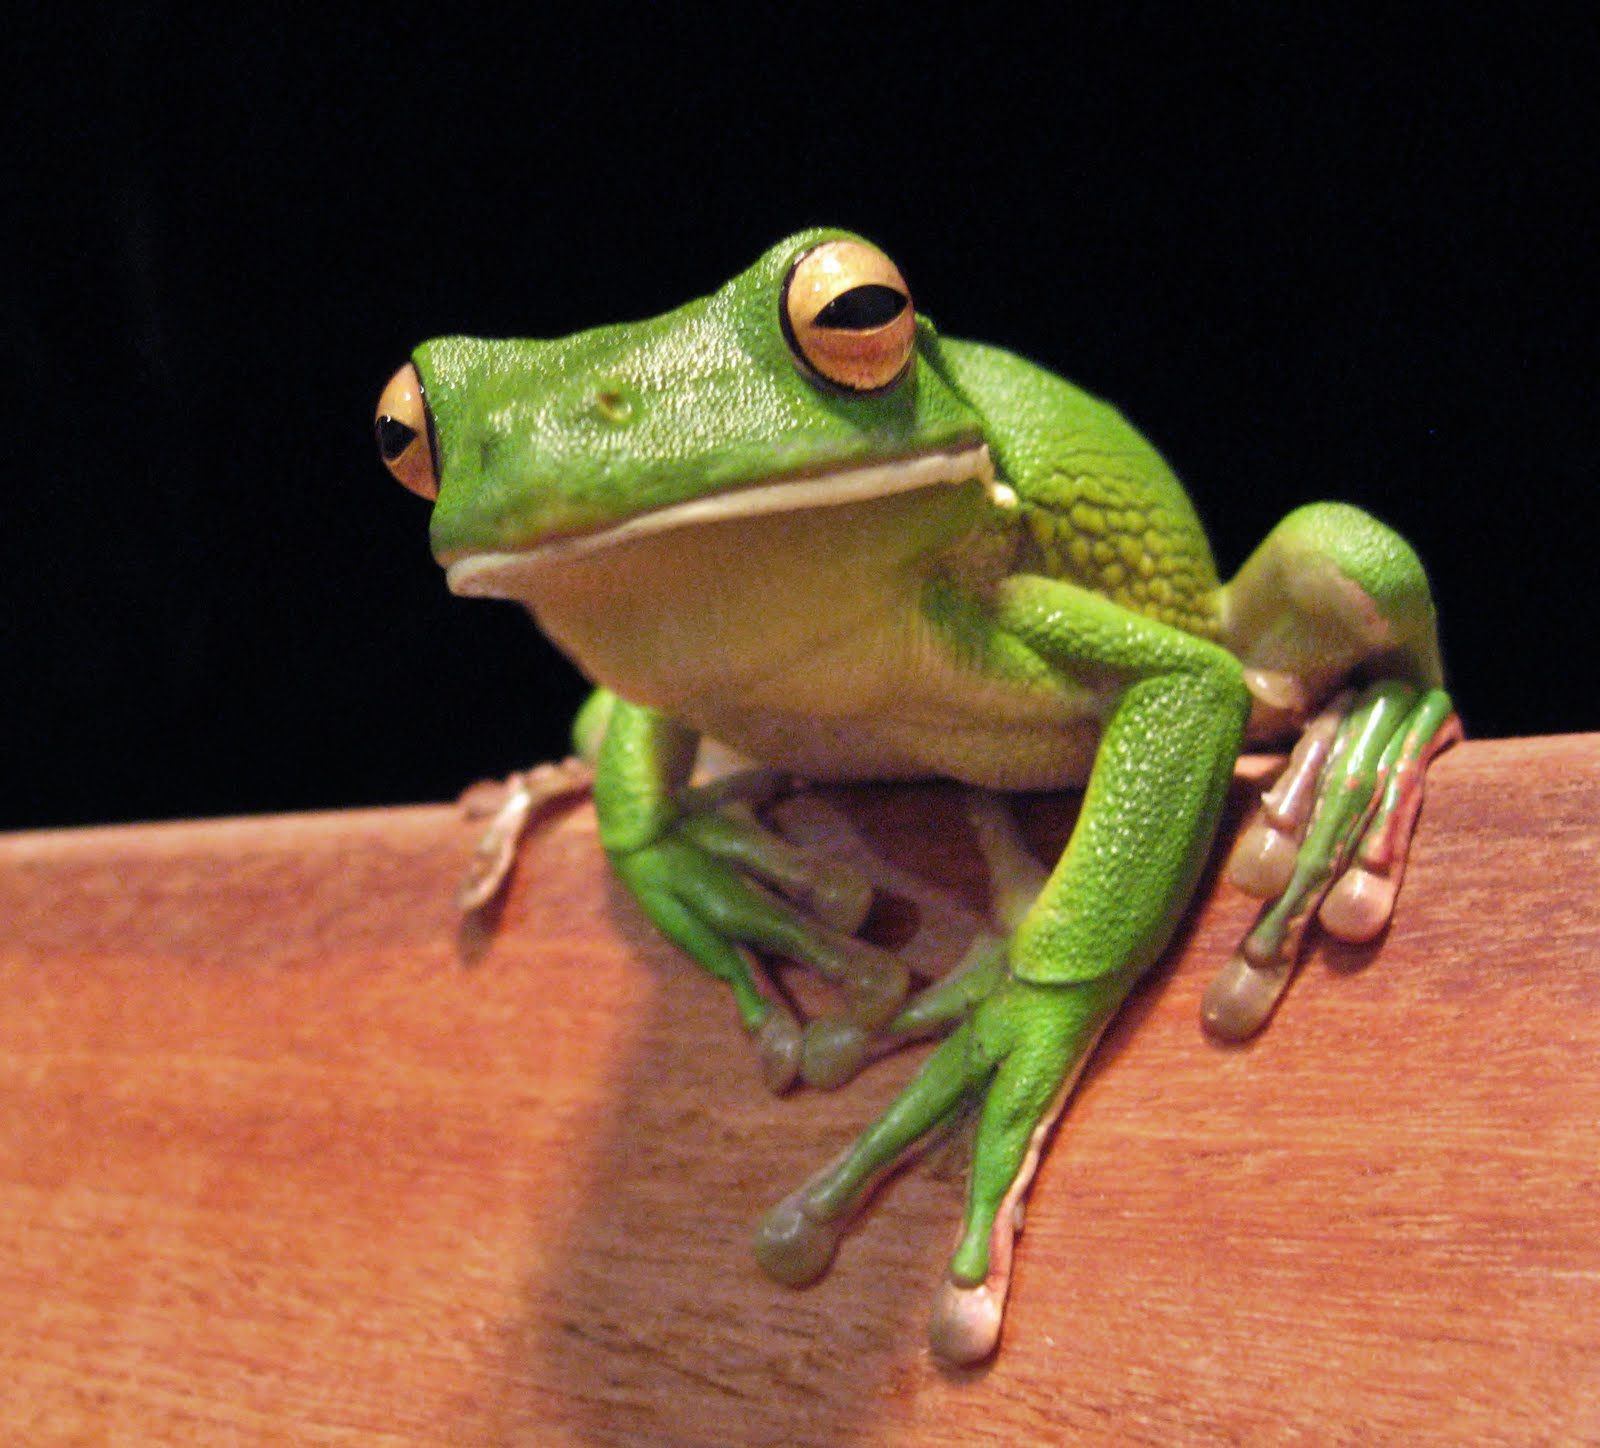
\includegraphics[width=0.25\textwidth]{frog.jpg}
	\caption{\label{fig:frog2}This is a figure caption.}
\end{wrapfigure}

\lipsum[2-3]

\end{document}